
\documentclass[12pt,a4paper]{article} 

\usepackage{float,times,graphicx,mathtools}
\usepackage{amsmath}
\usepackage{amsfonts}
\usepackage{amssymb}
\usepackage{latexsym}
\usepackage{epsfig}
\usepackage{graphicx}
\usepackage{caption}
\usepackage{subcaption}
\usepackage{color}
\usepackage{pdfpages}
\usepackage{natbib}
\usepackage[space]{grffile}
\usepackage{wrapfig}
\usepackage{subcaption}
\usepackage{url}
\usepackage{bbm}

\DeclareMathOperator{\logit}{logit}
\DeclareMathOperator{\tr}{tr}
\bibpunct[, ]{(}{)}{;}{a}{,}{,}
\graphicspath{{../}}  
\addtolength{\oddsidemargin}{-1in}
	\addtolength{\evensidemargin}{-1in}
	\addtolength{\textwidth}{1.75in}
	\addtolength{\topmargin}{-1.3in}
	\addtolength{\textheight}{2in}
\date{\vspace{-5ex}}
\begin{document}

\begin{itemize}
\item Estimated gx seems crazy after age 75 in the early years (e.g. in 1960-1964 for females aged 75-79 estimated gx is $\approx -0.7$)
\item Currently assumed RW on $h_t$ and $k_t$ of the LogQuad Model for males and females independently, will try to introduction some correlation between the two sexes. 
\item the huge difference in estimated $_{45}q_{15}$ at the earliest years is due to the much higher estimated RW penalty on female $k_t$, while for males $k_t$ are allowed more flexibility hence closer to the empirical sx
	\begin{itmeize}
	\item[\arrow] magnitude of the estimated gx of both sexes in these years are similar, but estimated gx are $+ve$ at age 40-59 for males and $-ve$ for females
	\item[\arrow] gx over-compensated for males to allow for higher mx to match empirical sx for males, or gx under-compensated for mx to be more similar across years for females
	\item[\arrow] assume common RW penalties in $h_t$ and $k_t$ across sexes?
	\end{itemize}
\item Compared estimated mx in 1990-2015 to those from only using DHS-Spline, estimates from the CCMPP-LogQuad Model with DHS deaths are generally higher
\item Only 5x5 age-period grid have been considered so far, will try to interpolate the LQ Model to single year of age.
\item Simple MVN on migration rates at the moment, will try to introduce correlation soon (age and time direction or time and cohort direction?). Penalty on gx such as tensor P-spline penalties?
\item RW on tips, will add spikes at tips=5 and tips=10
\end{itemize}

\paragraph{LogQuad Model} \\~\\
\begin{align*}
\log (m_{x,t}) = a_x + b_x h_t + c_x h_t^2 + v_x k_t
\end{align*}
where $a_x, b_x, c_x$ and $v_x$ are fixed coefficients.

Obtained coefficients from the package \textit{MortCast} which contains the coefficients of the LogQuad Model at age groups $0, 5\text{-}9, 10\text{-}14, \dots, 110\text{+}$. Age group $1\text{-}4$ are left out as in the original LQ Model the $_4q_1$ are calibrated such that the modelled $p_0 \, _4p_1$ match the input $_5q_0$. 

Coefficients starting at age group $5\text{-}9$ were extracted and the log mortality of the first age group $0\text{-}4$ was set to be the estimated $h_t$.
 
AR(1) is assumed on $h_t$ and $k_t$ for both males and females, independently.

The open age group in the population counts data starts at a younger age than the LQ Model, therefore weighted average of the estimated mortality rates of the last few age groups are calculated, with weights equal to the exposures according to the life table assuming UDD.

\newpage
\paragraph{Results} \\~\\

\begin{figure}[H]
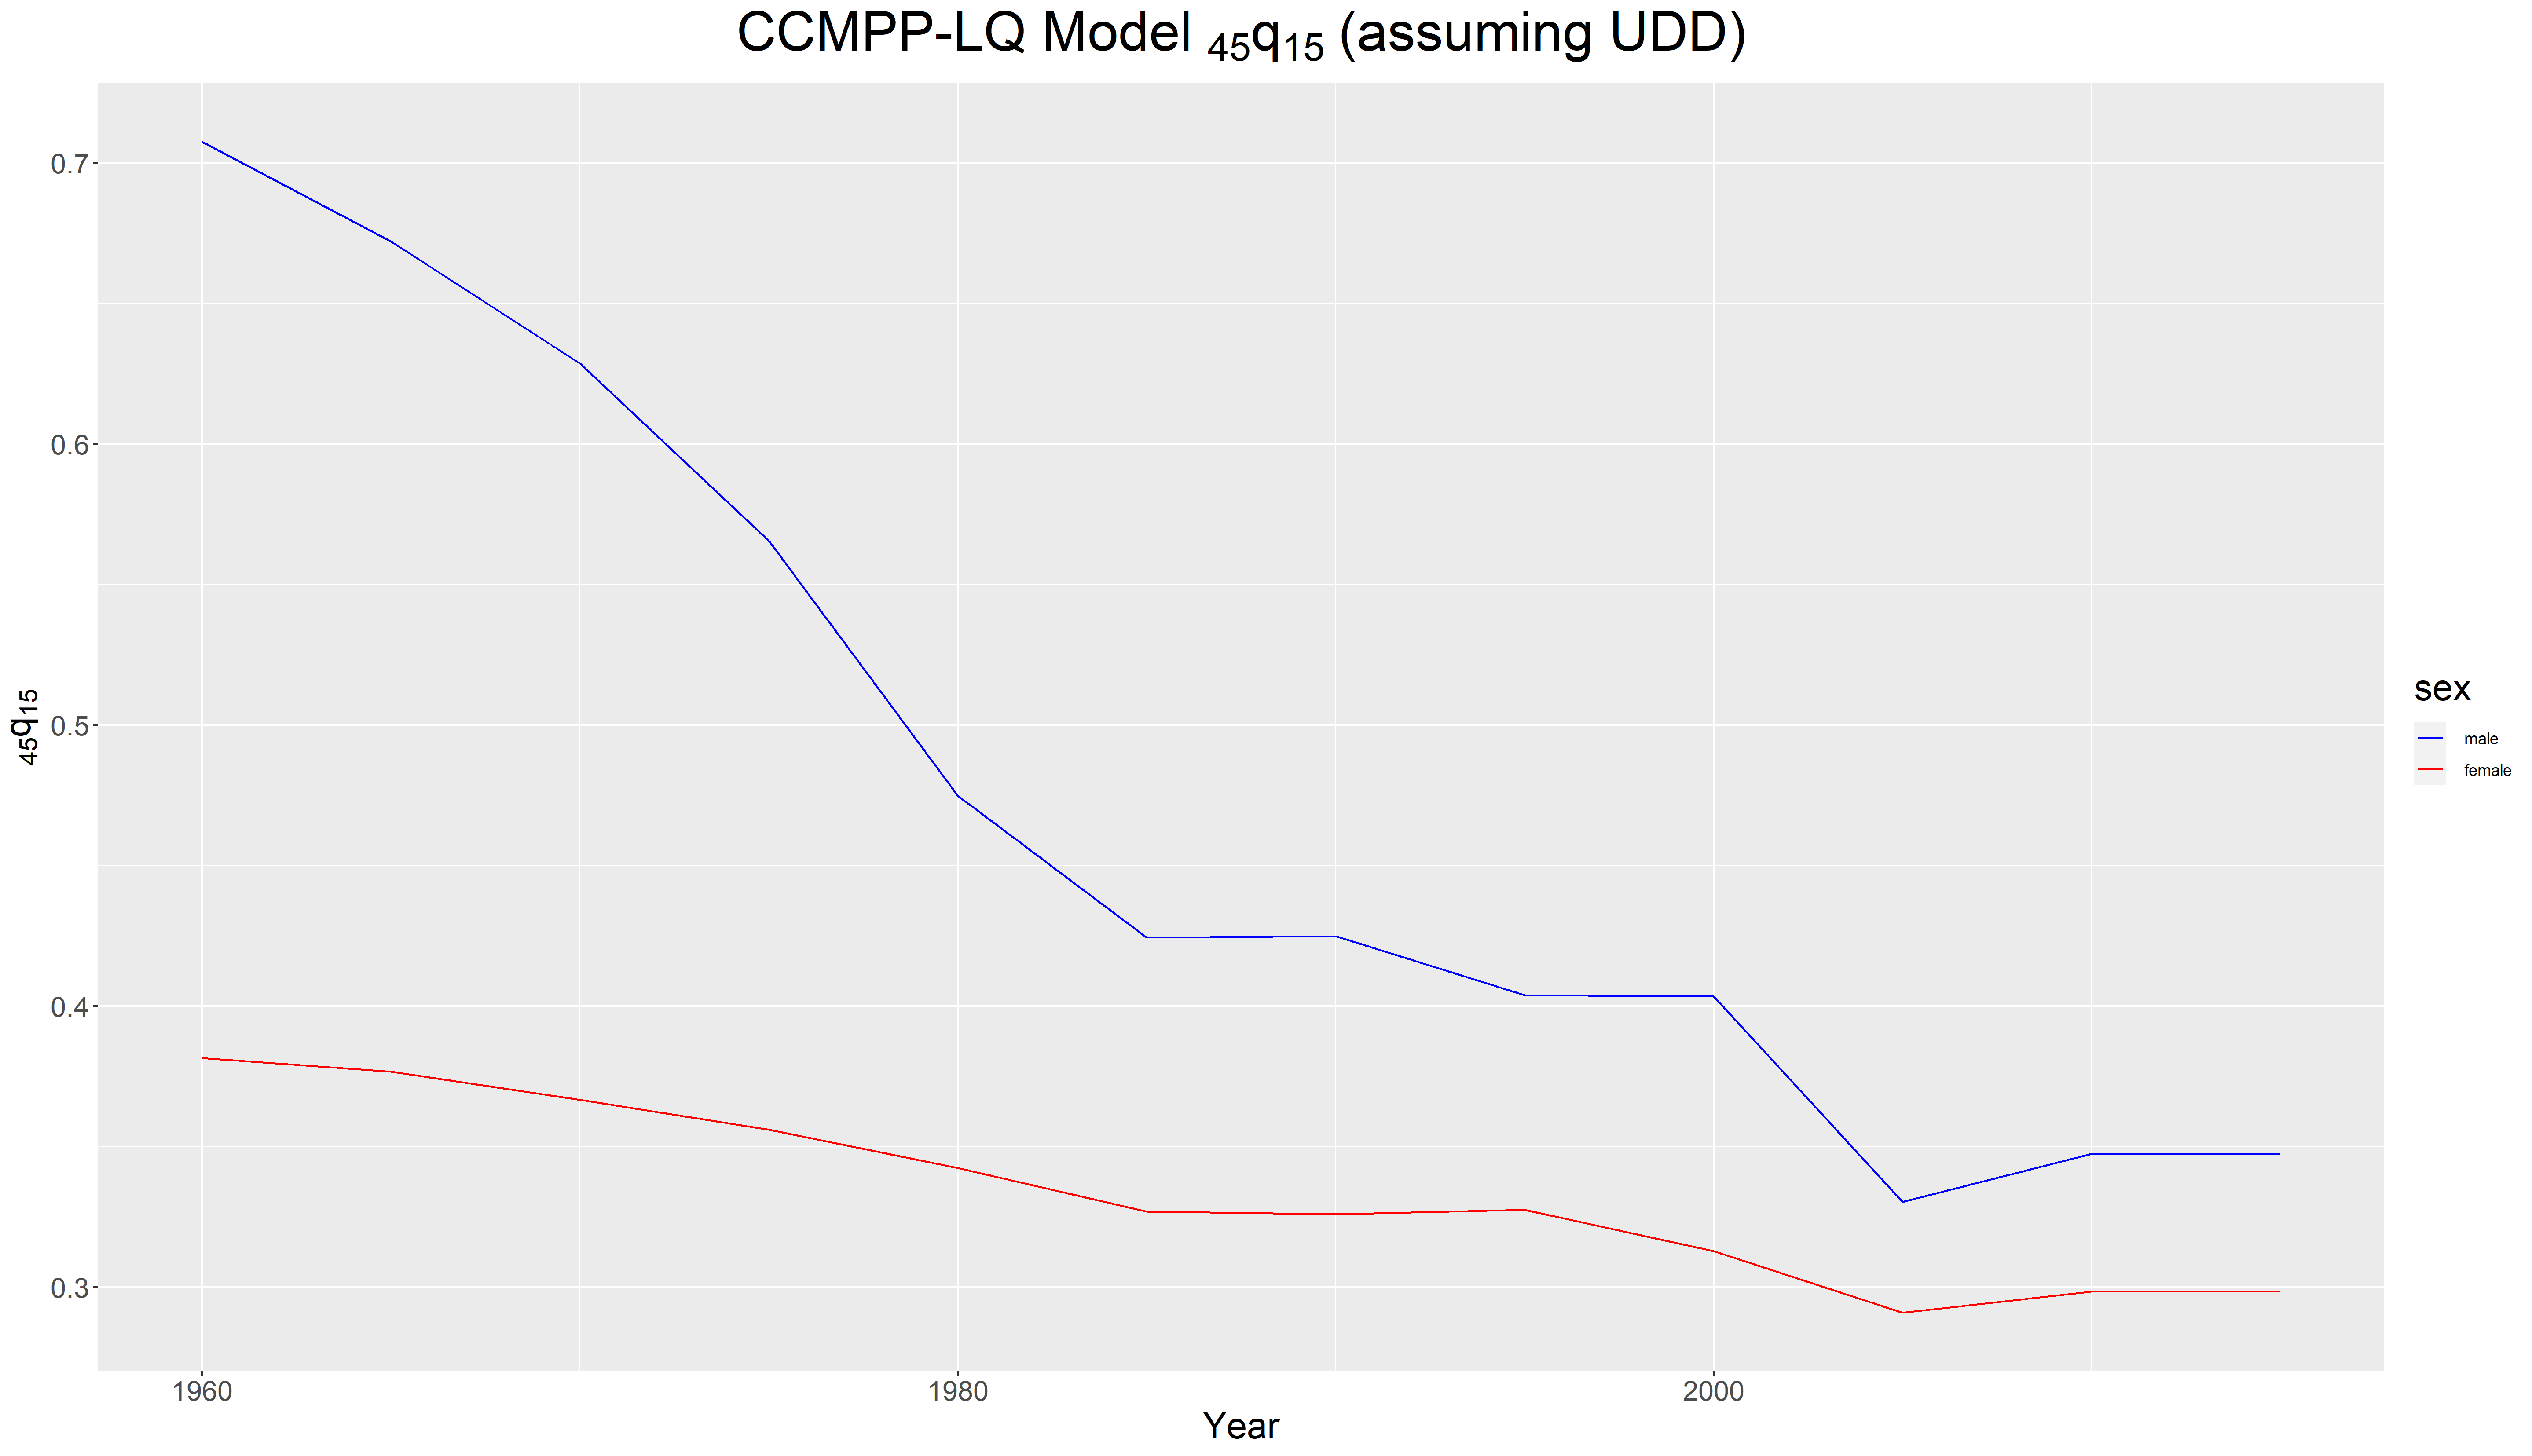
\includegraphics[width=\linewidth]{Burkina Faso/CCMPP q4515.png}
\end{figure}
\begin{figure}[H]
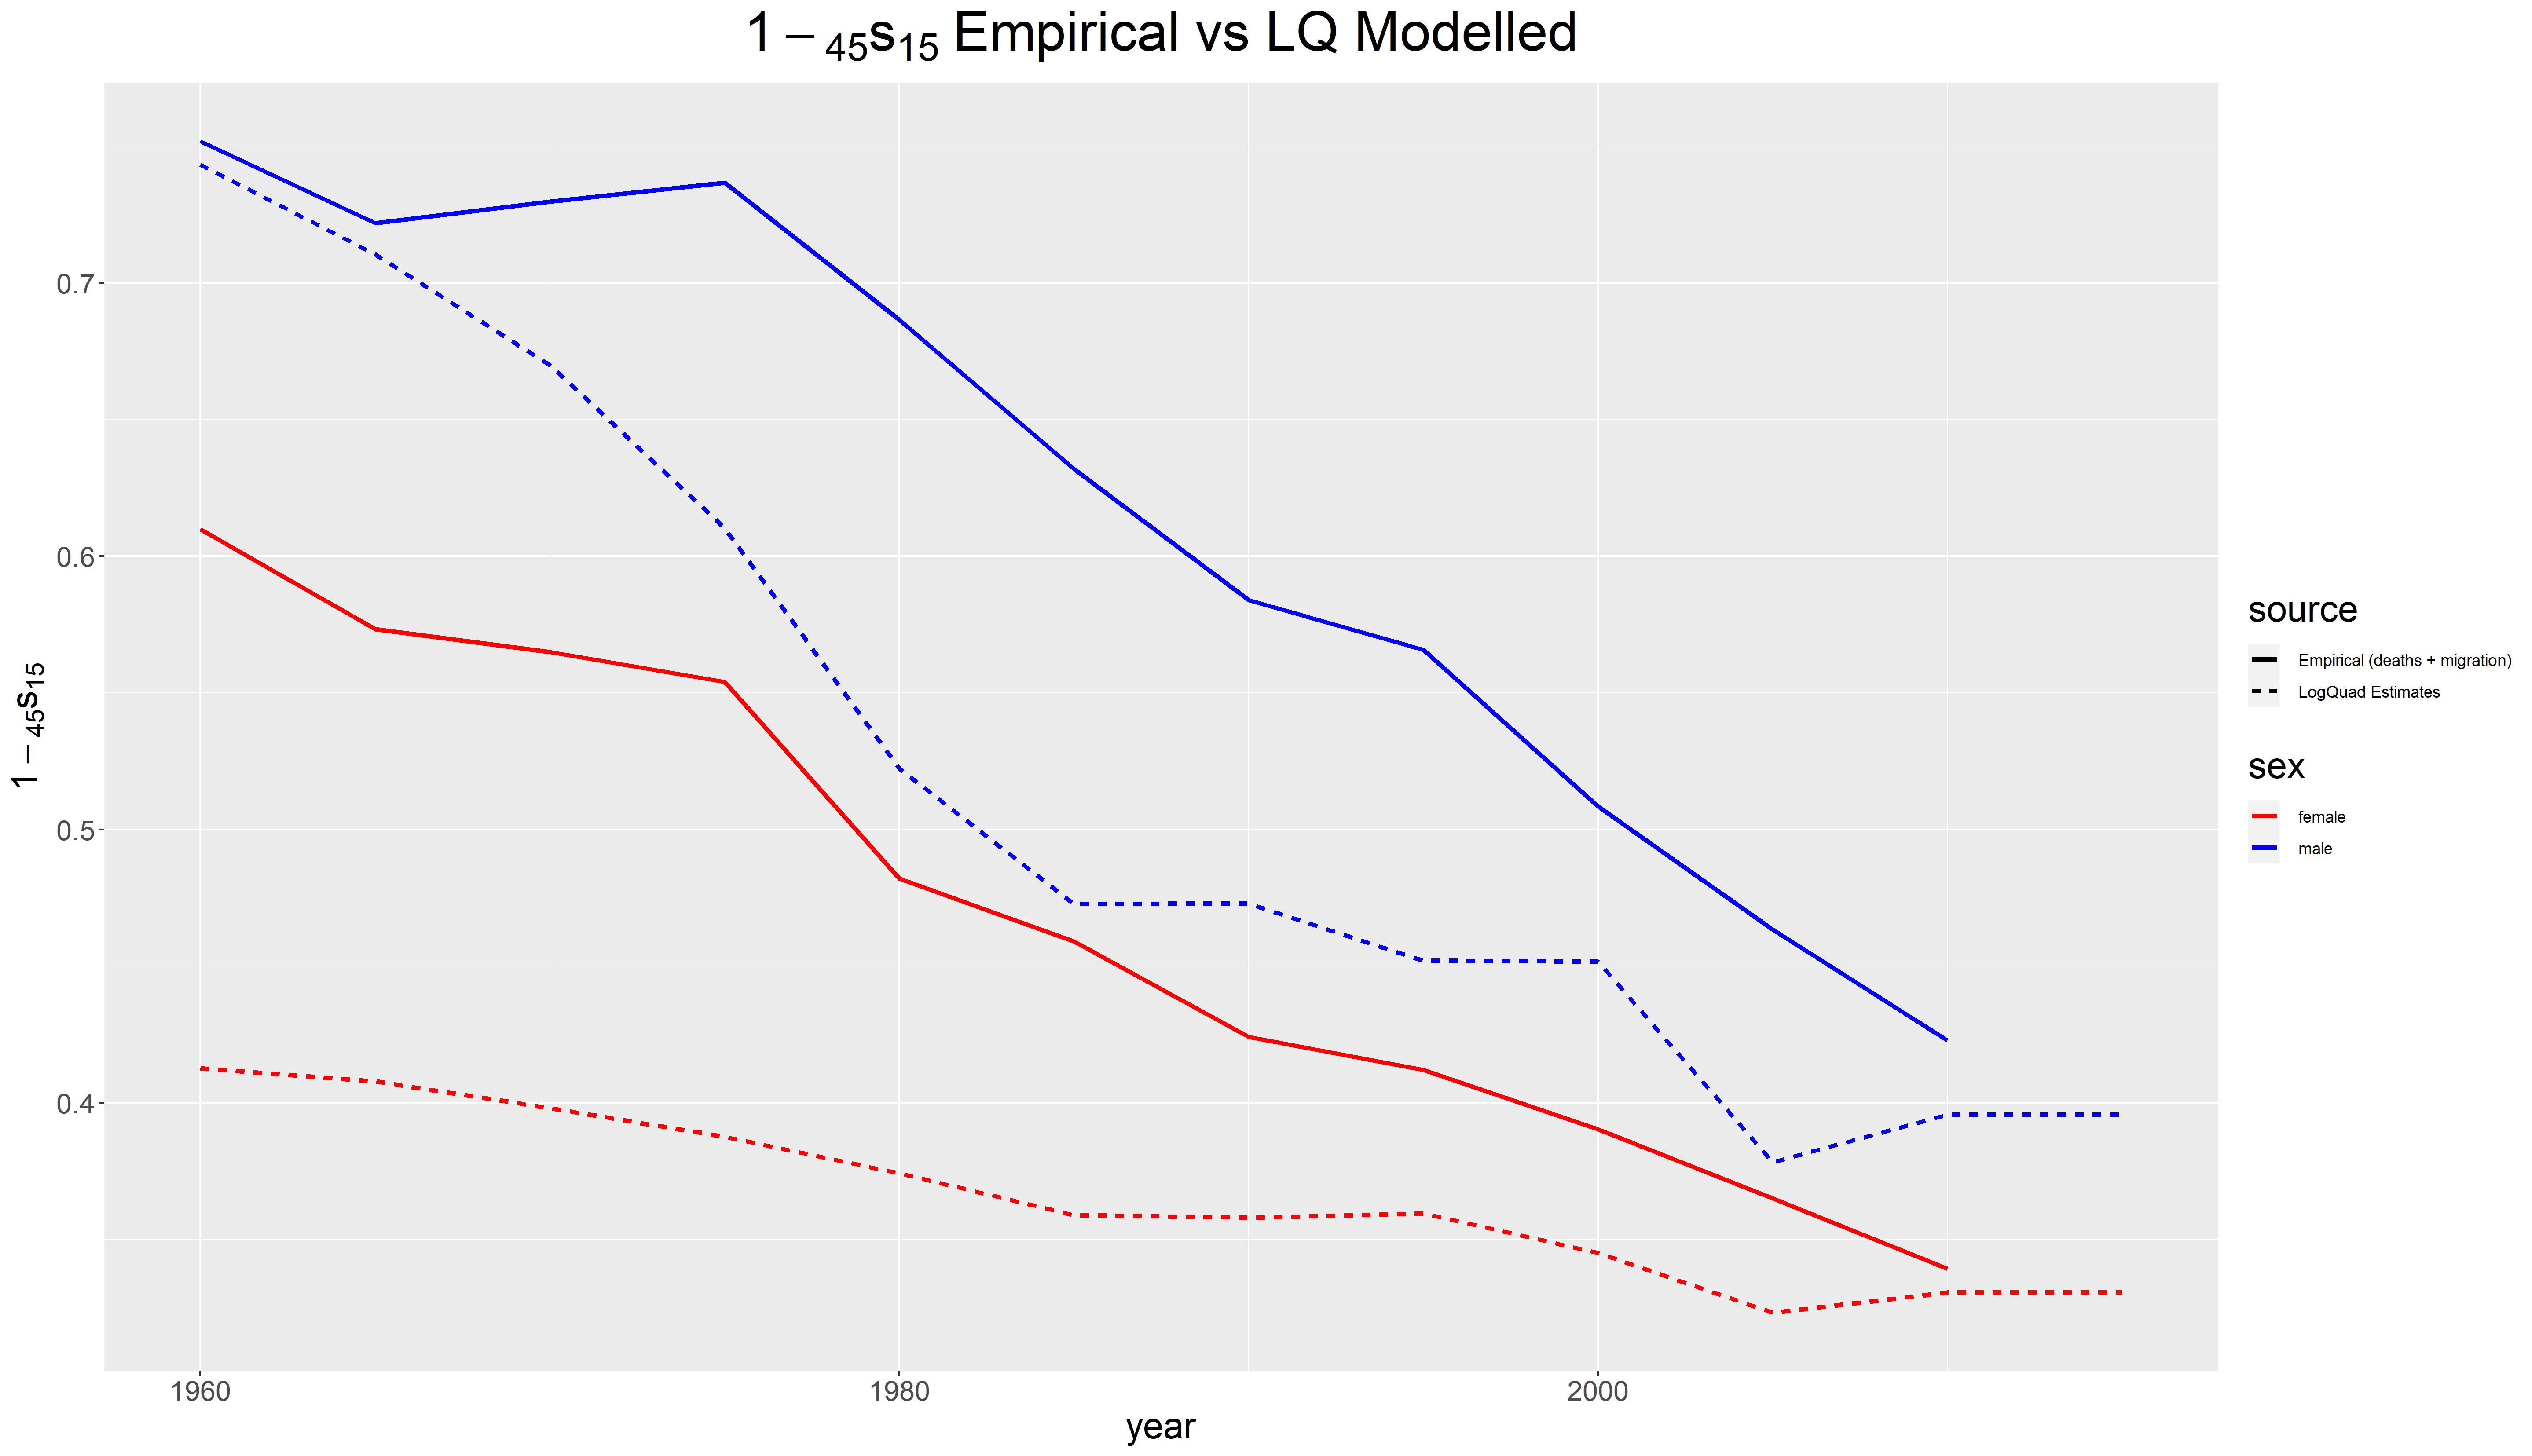
\includegraphics[width=\linewidth]{Burkina Faso/CCMPP 1-s4515.png}
\end{figure}

\begin{figure}[H]
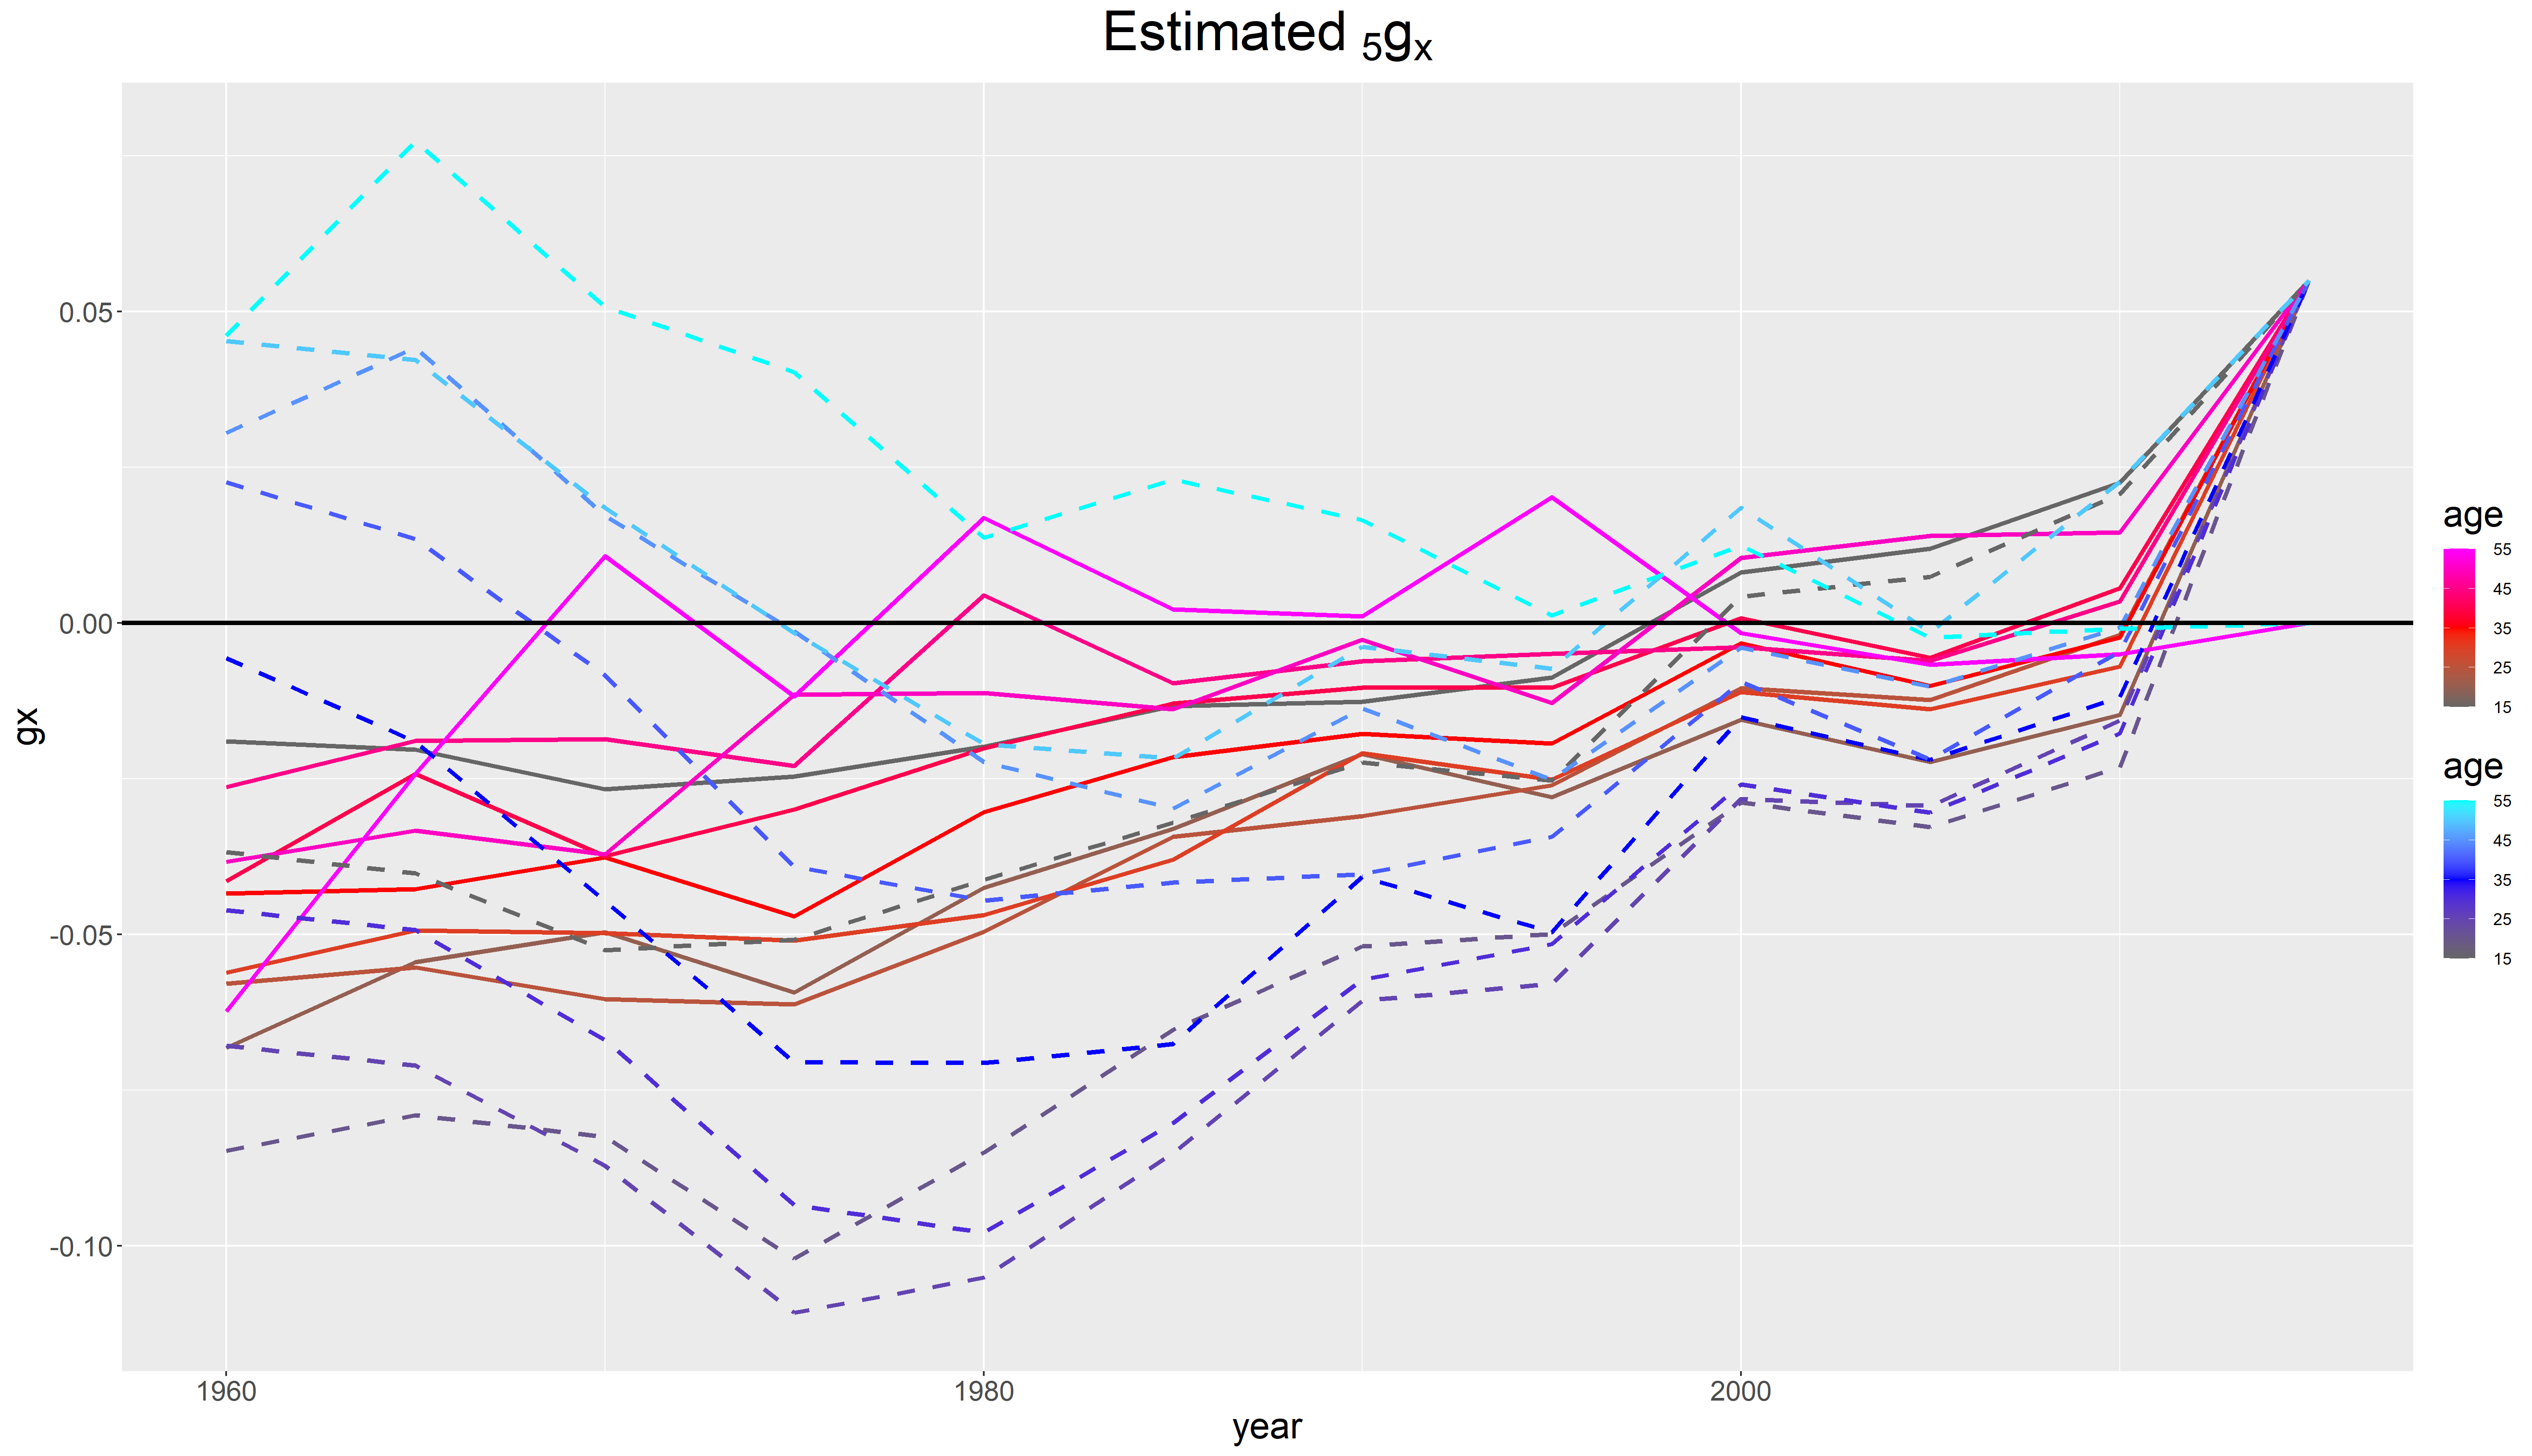
\includegraphics[width=\linewidth]{Burkina Faso/gx 15 to 60.png}
\end{figure}

*Prior for gx set to -0.055 at most of these ages

\newpage
\paragraph{Comparison to DHS-Spline} \\~\\
\begin{figure}[H]
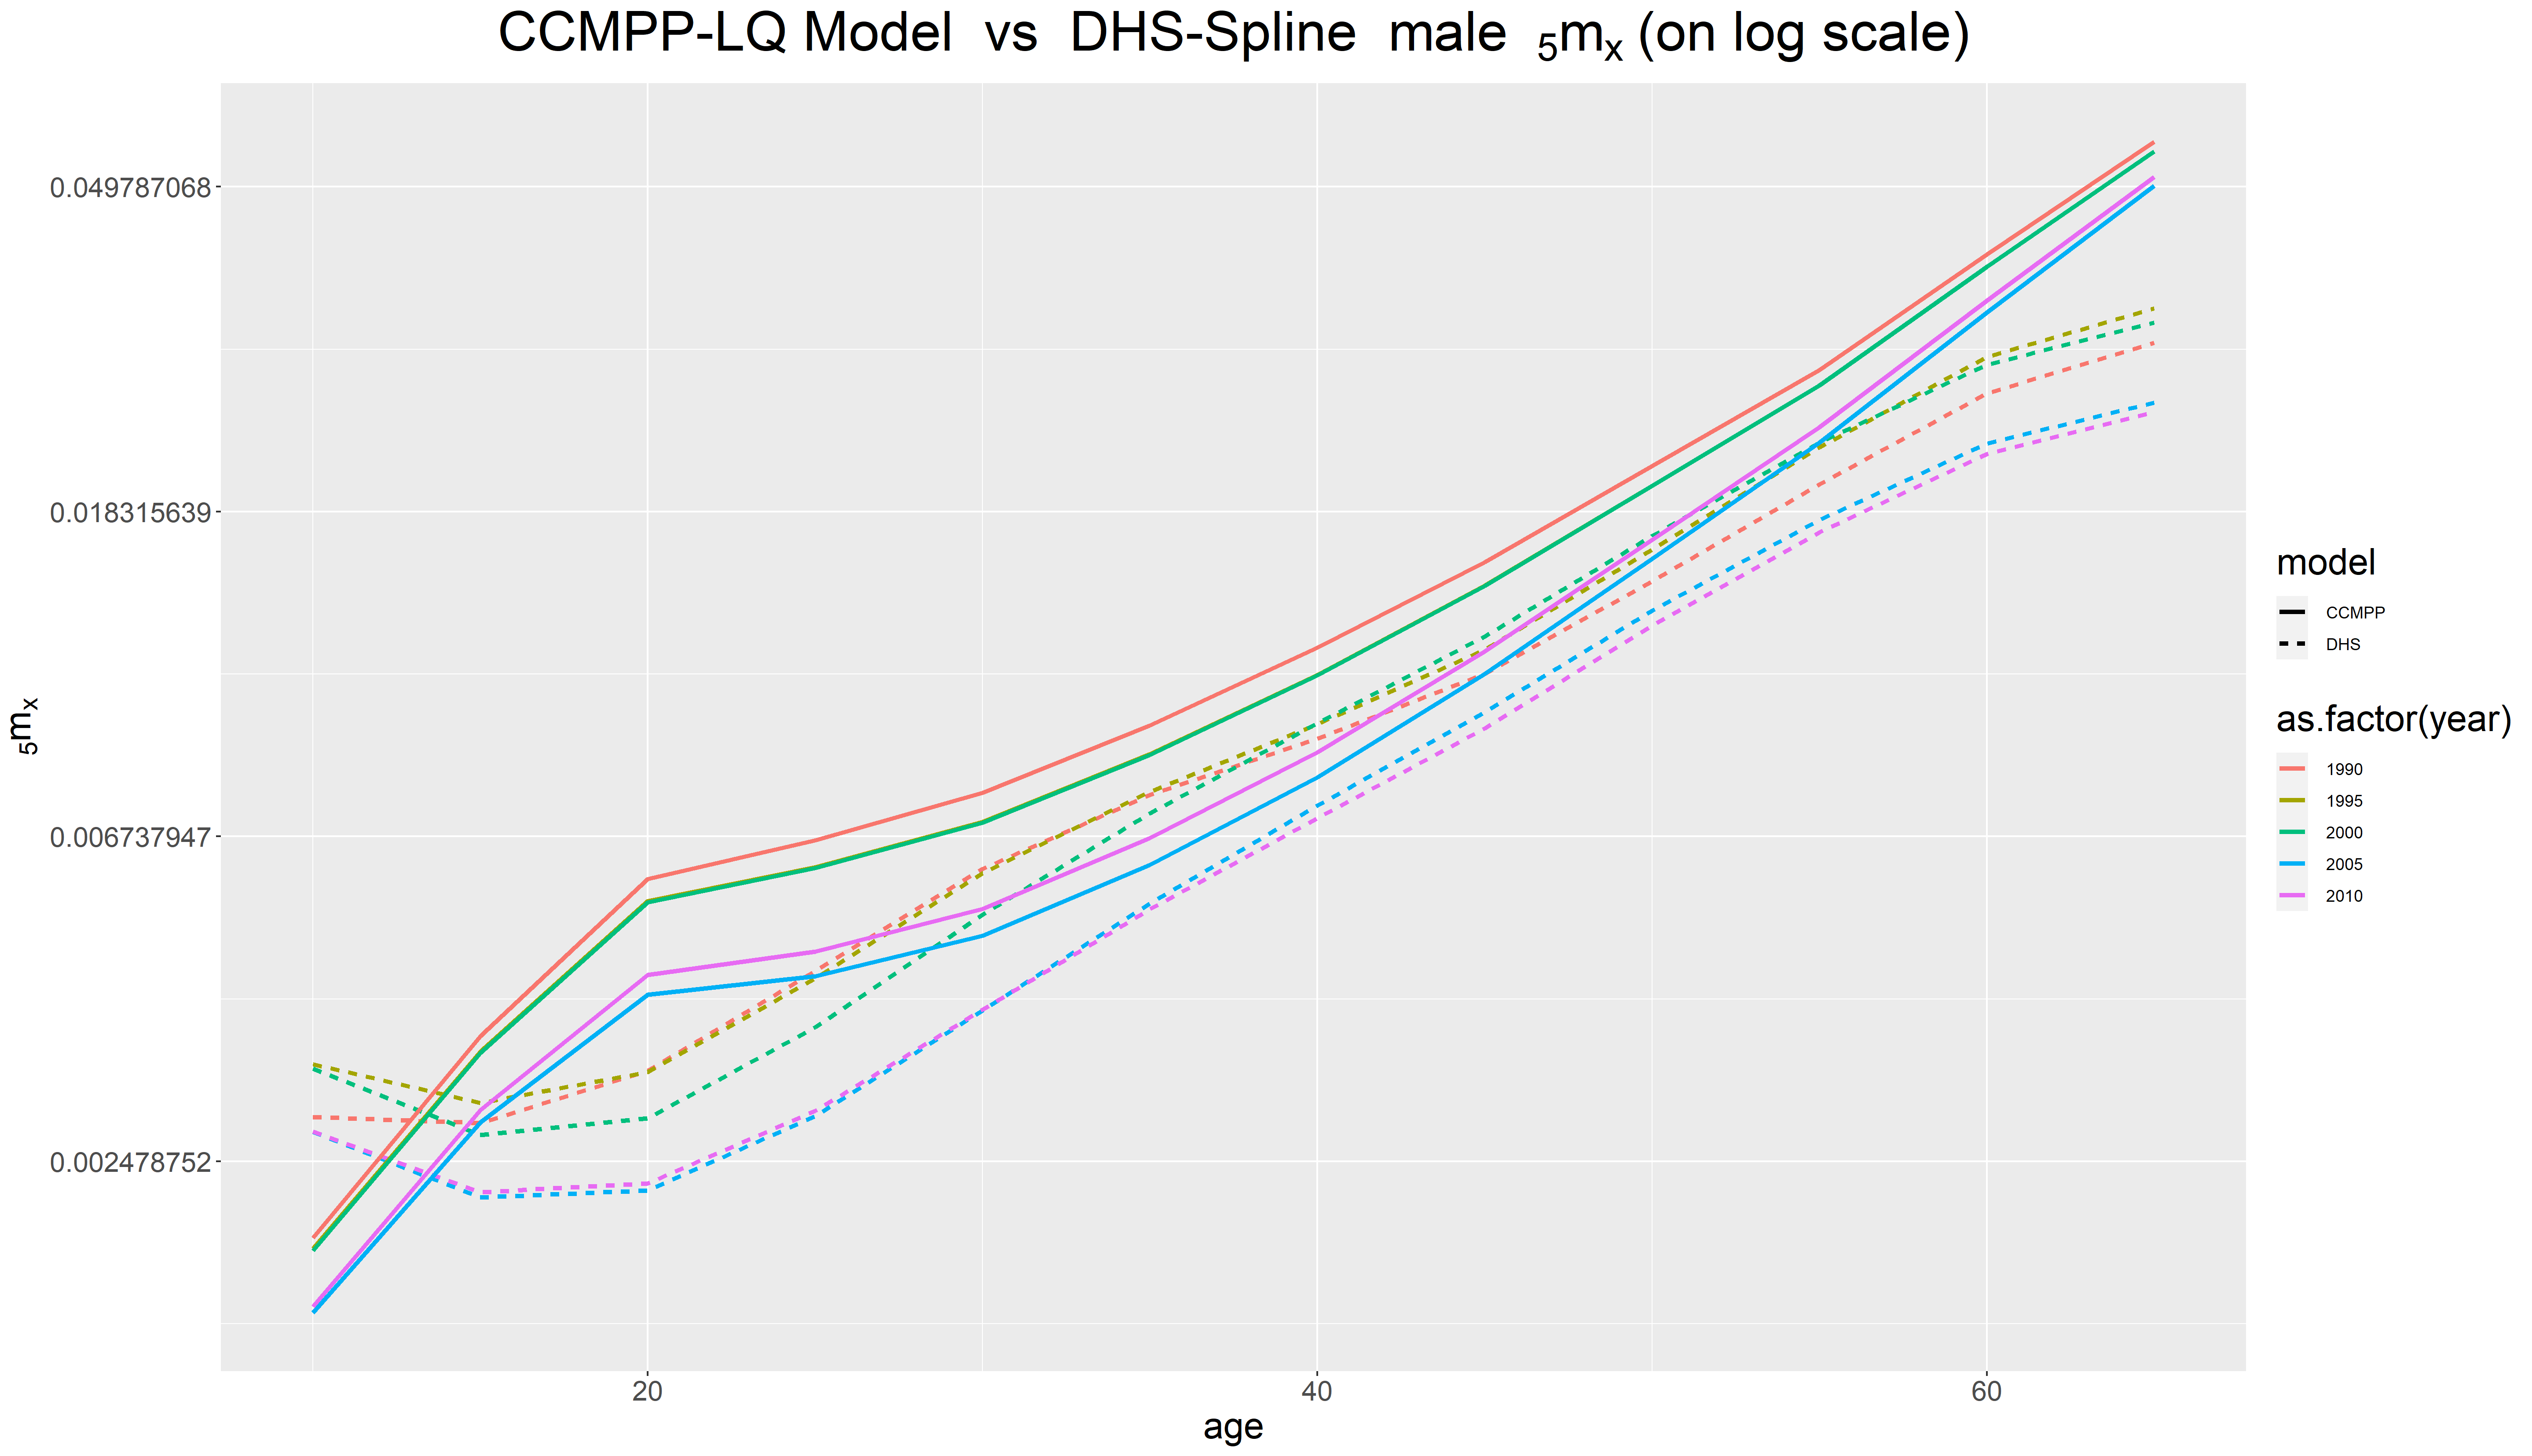
\includegraphics[width=\linewidth]{Burkina Faso/compare DHS males year.png}
\end{figure}
\begin{figure}[H]
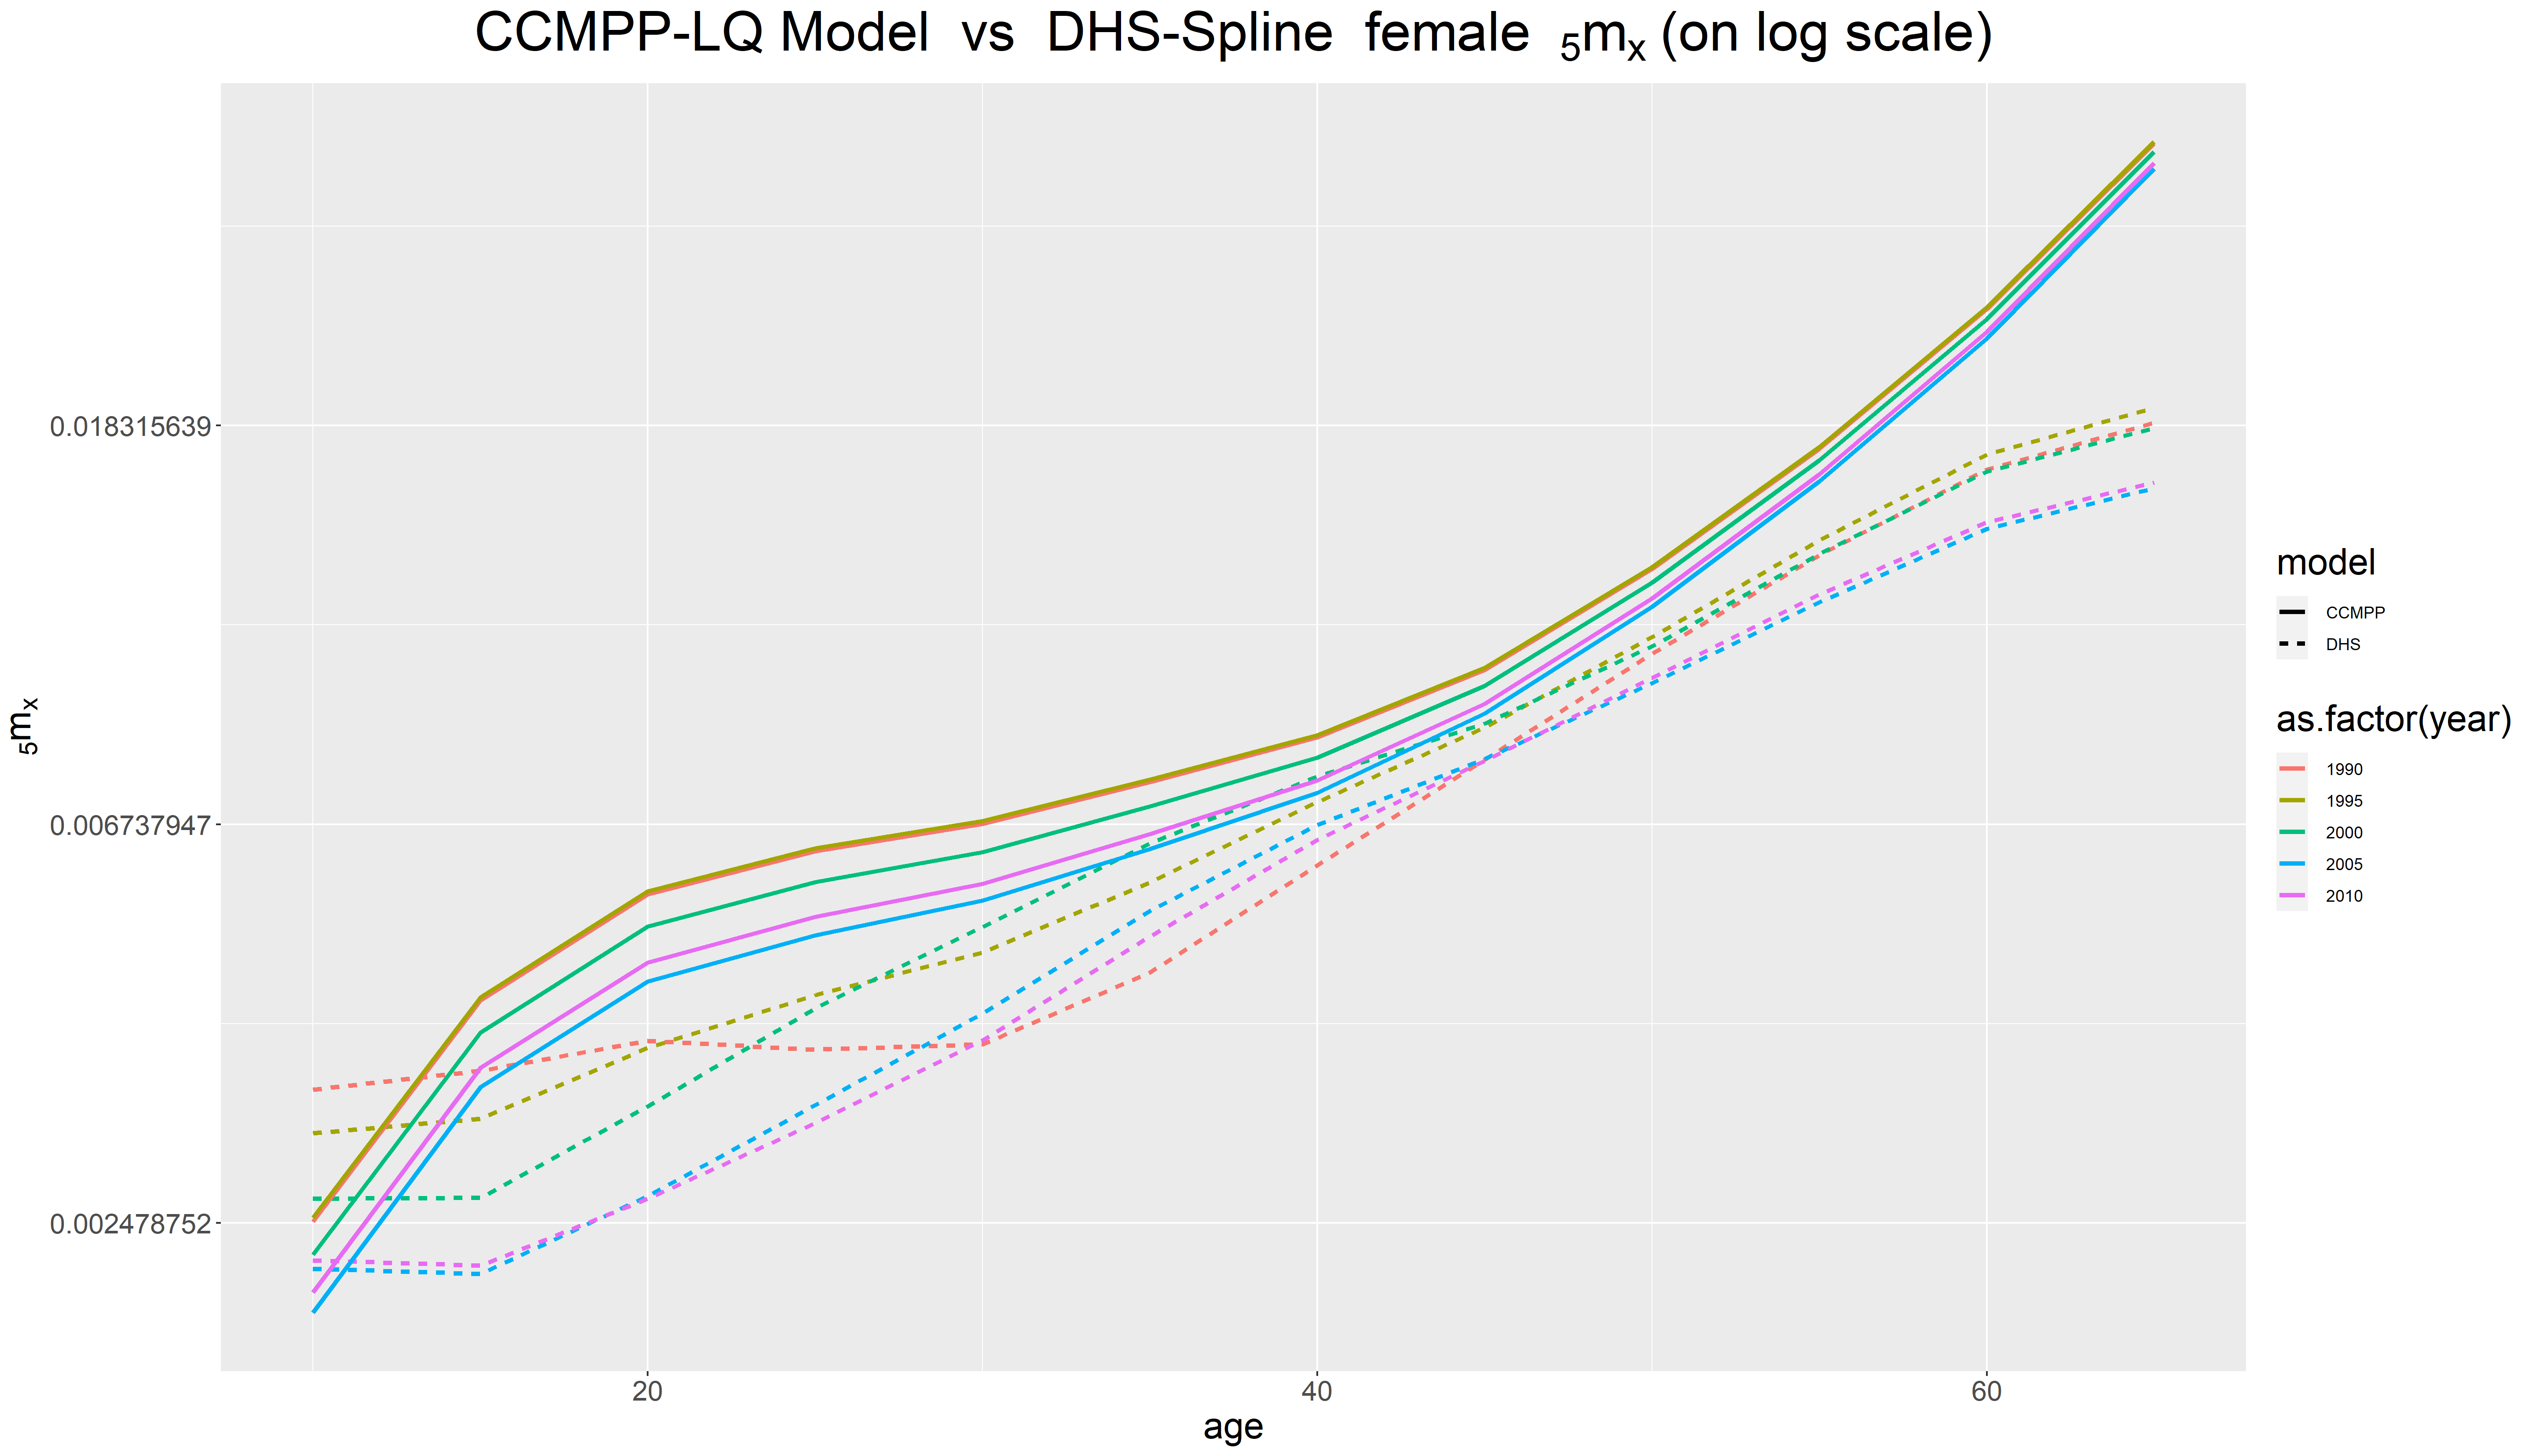
\includegraphics[width=\linewidth]{Burkina Faso/compare DHS females year.png}
\end{figure}

\begin{figure}[H]
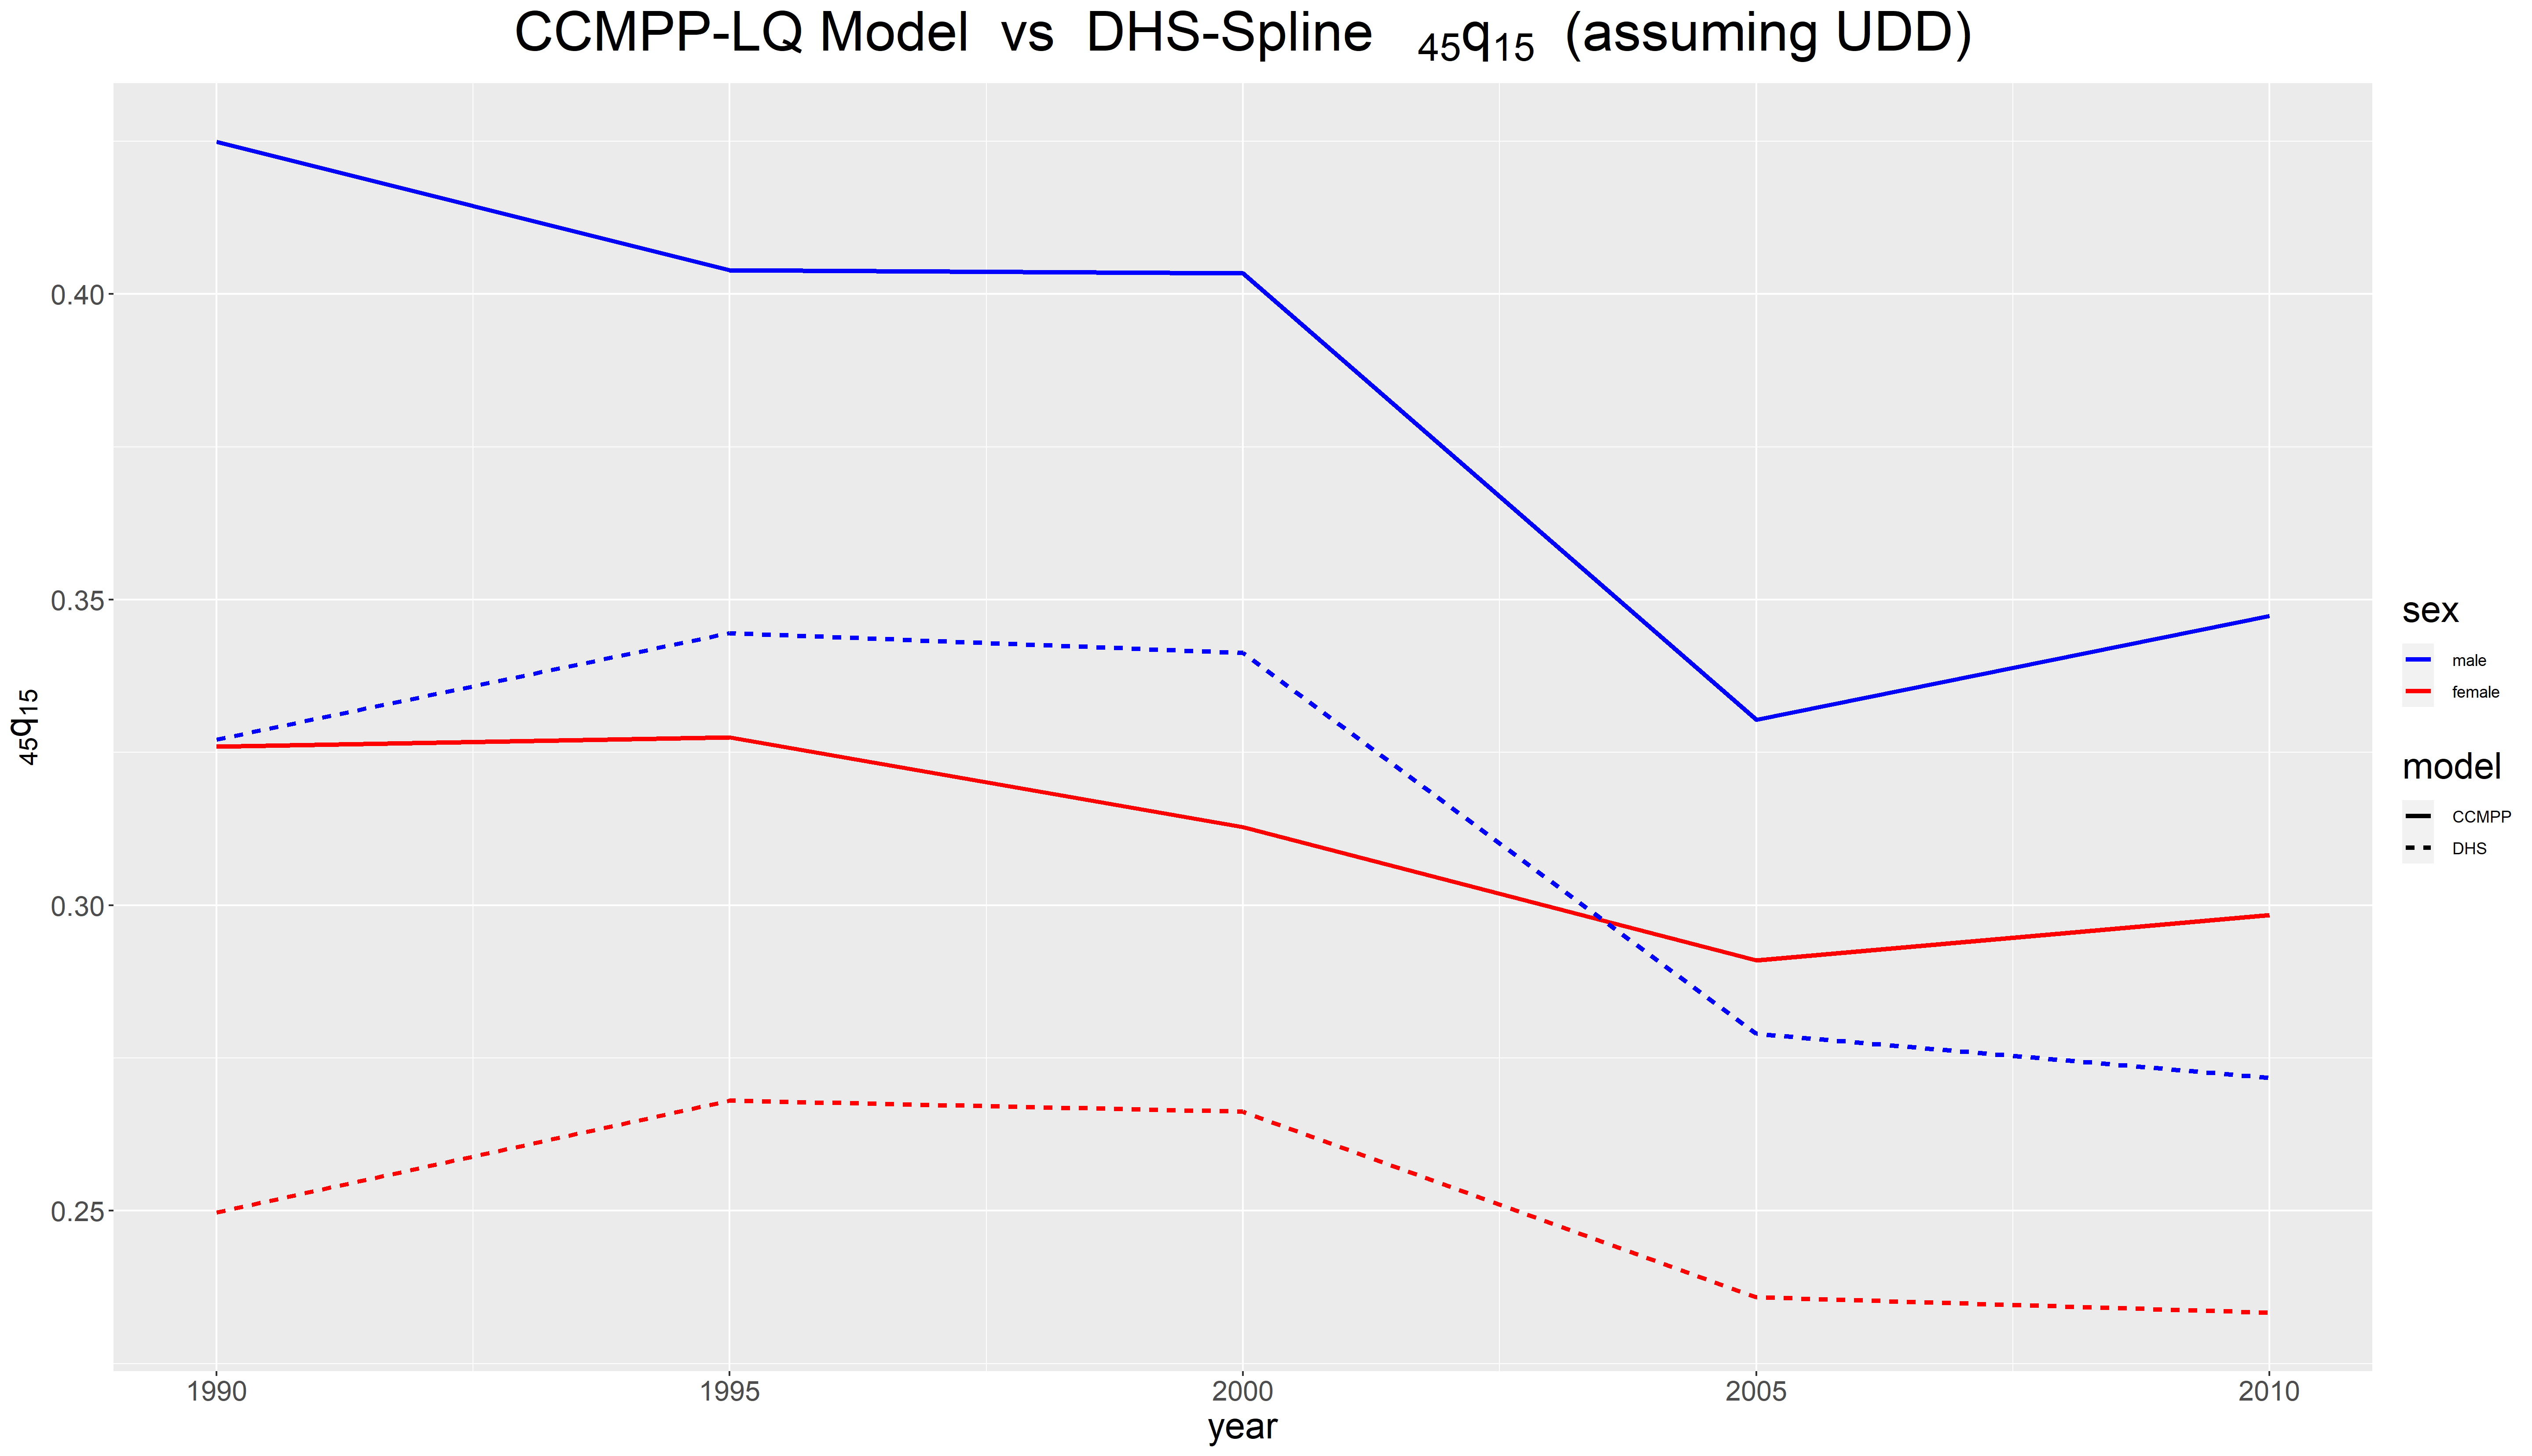
\includegraphics[width=\linewidth]{Burkina Faso/compare DHS q4515.png}
\end{figure}
\end{document} 